\documentclass[12pt, fullpage,letterpaper]{article}

% I copied older latex files that include packages we may need but idk,
% I'm not too knowledgeable about all things Latex
\usepackage[margin=1in]{geometry}
\usepackage{url}
\usepackage{amsmath}
\usepackage{amssymb}
\usepackage{xspace}
\usepackage{graphicx}
\usepackage{hyperref}
\usepackage{listings}
\usepackage{bm}
\usepackage{cite}
\usepackage{subfigure}

\graphicspath{{./}}
\title{Progress Report}
\author{Tyler Adams: u0761872 \\Corbin Baldwin: u0292800}

\begin{document}
	\maketitle 
	\hrule 
	\vskip 0.5cm
	\section*{\normalfont Introduction}
	% Motivation and a brief project description.
	Rayleigh-Taylor instability (RTI) forms at the surface of contact between two fluids, one of which is denser and accelerates toward the other. Formations in RTI are not symmetric between the denser and lighter fluids, and the features of both sides serve to characterize the RTI. However, these features quickly rise in complexity, and it is unrealistic to simulate them beyond a given time threshold. In our project we hope to provide insights regarding structure that apply to RTI generally, including in the later stages of RTI development, using TDA methods.
	
	\section*{\normalfont Completed Milestones} We have successfully been able to install and run software that simulates RTI and saves the time-steps in images which we can use further down the pipeline. Additionally, we have written software that extracts the isosurfaces of the images with which we can track bubble evolution. An example time evolution is shown below.
		\begin{figure*}[ht!]
		\centering
		\begin{subfigure}
			\centering
			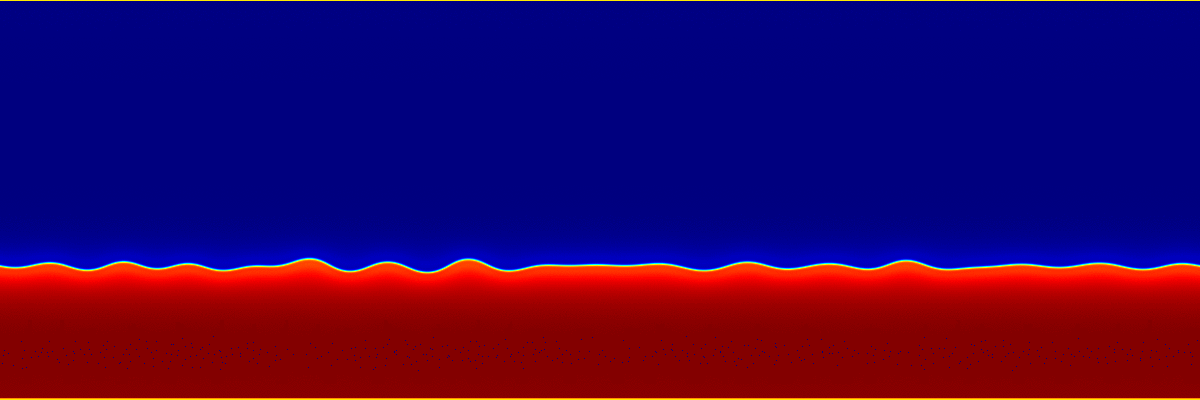
\includegraphics[scale = .3]{fig1.png}
			\caption{$t = 2100$}
		\end{subfigure}
		\begin{subfigure}
			\centering
			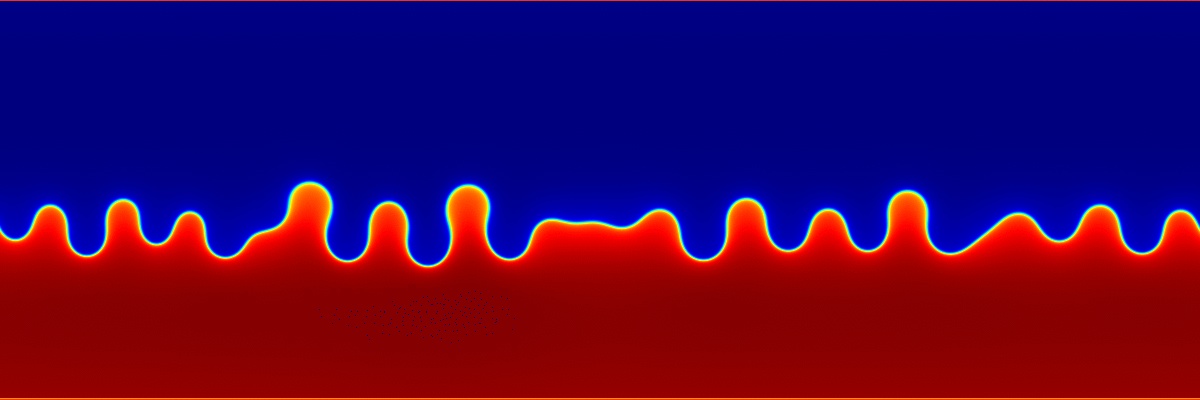
\includegraphics[scale = .3]{fig2.png}
			\caption{$t = 2600$}
		\end{subfigure}
		\begin{subfigure}
			\centering
			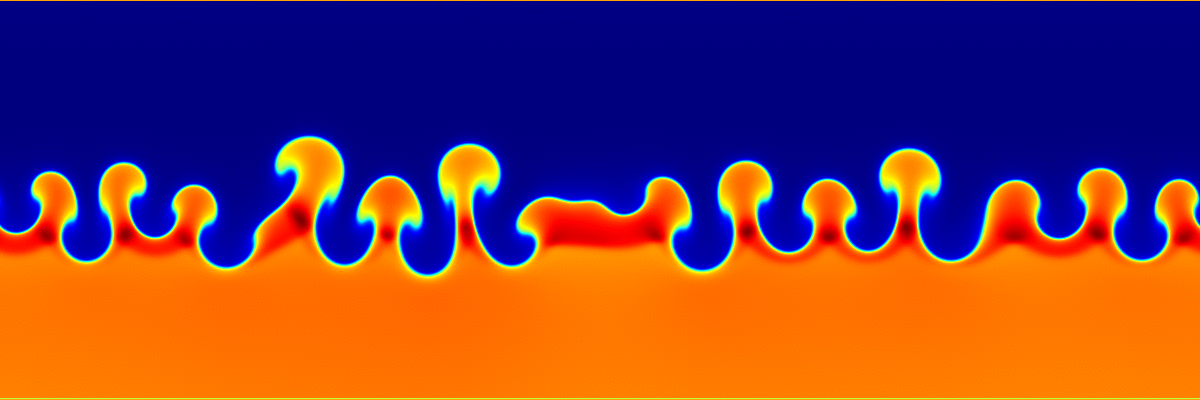
\includegraphics[scale = .3]{fig3.png}
			\caption{$t = 2900$}
		\end{subfigure}
		\begin{subfigure}
			\centering
			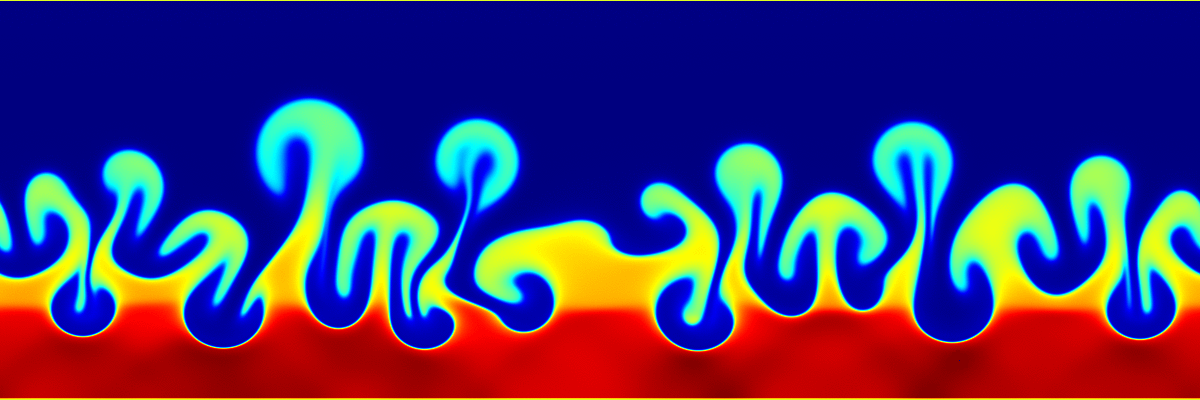
\includegraphics[scale = .3]{fig4.png}
			\caption{$t = 3300$}
		\end{subfigure}
	\end{figure*}
	
	
	\section*{\normalfont Upcoming Milestones} The next milestones are:
	\begin{enumerate}
		\item Smooth out the isosurfaces so that we can better track bubble evolution.
		\item Implement a height function to track critical points and the evolution of bubbles.
		\item Construct a persistence diagram describing the birth and death of bubbles.
		\item Possibly classify simulations by density or other parameters by their persistence diagrams. I.e., is this bubble evolution symptomatic of the mixing of air and water?
	\end{enumerate} 

	\section*{\normalfont Preliminary Results}
	While we have not applied a proper topological filtration, we have extracted some data that will be necessary in the final stages. The most challenging aspect so far has been finding a valid, practical algorithm for running the simulation of an RTI. As shown above, we have managed to get one working that provides a solution to the problem in the two dimensional case. With the images that are output, we can approximate the isosurface using edge-detecting algorithms, which we have done.
	
	\section*{\normalfont Modifications}
%	Originally, we planned to study three dimensional RTIs, but it appears that this may be impractical with the computing power available to us. The two dimensional case may be simplified, but it also allows us to study the fluctuations with more detail, as we can observe the interiors of each bubble. 
	
	\section*{\normalfont Summary}

%  
%	\section*{\normalfont Project Objective}  
%%	What is the main objective/goal of your project?  What are you planning to
%%	do to achieve your objective/goal?
%	In this project, we plan to explore various topological filtrations of RTI data to expose meaningful properties of the RTI. RTI is at a stage of development in which there are few, if any, application inspired motivations in its research. Instead, researchers in fluid dynamics simply seek to understand it more extensively. We hope to describe the structure of the formations in RTI using TDA techniques.
%	
%	\section*{\normalfont Data} 
%%	What are the type(s) of data your project will be dealing with?  How do you plan to get hold of such data sets?  What kind of insights are you planning to obtain from your data?
%
%	Our dataset has to be simulated using the physics of bubble formation as briefly described in the introduction. In particular, we will use a set of points in $\mathbb{R}^3$ that also have viscosities and velocities. In \cite{paper}, hereafter referred to as the paper, the authors had access to a supercomputer, a resource that we do not have, so we must generate a significantly smaller simulation. Instead of the $1152^3$ or $3072^3$ data points, we will use $256^3$ points. The reason for simulation stems from the obvious difficulty in precisely measuring bubble formation and maturation.
%	
%	\section*{\normalfont Background} 
%%	What are the state-of-the-art techniques in dealing with the data of your interest?
%	Studying the bubble interactions of RTI is a relatively new practice, but the perhaps the most successful method to date involves Morse-Smale complexes. Indeed, the inspiration for this research, the work by Laney et al. is centered on producing MS-complexes over the bubbles formed in RTI. Our work will involve a component of this as well.
%	
%	One problem with MS-complexes in this context is that they only capture still moments. There is a general feature tracking algorithm proposed by Samtaney et al. that connects features such as bubbles across time, resulting in a graph. Similarly, one can compute time-varying Reeb graphs of RTI.
%	
%	  
%	\section*{\normalfont Technical Contributions} 
%%	What are the expected technical contributions of your proposed work?
%%	What are the differences and similarities between your proposed work and the state-of-the-art?
%	In addition to analyzing RTI with MS-complexes, we will introduce modified topological filtrations in an attempt to extract additional information related to the RTI. For example, we will consider the topology of the level sets parallel to the surface of contact between fluids.
%
%	
%	
%	\section*{\normalfont Expected Outcomes and Deliverables}  
%%	What are the expected outcomes of your proposed project?
%%	What do you plan to hand in?  (e.g.  source code, video demo, etc.)
%We expect to be able to reproduce the results of the paper, albeit with a significantly smaller dataset. In addition, we expect that different filtrations (by using different complexes other than Morse-Smale) as well as utilizing different Morse functions will extract meaningful information. More precise expectations will come forward when we decide which specific filtrations and  Morse functions to use. Our hand-in will consist of source-code and visualizations of our results. Specifically, the visualizations will include a graph showing birth-death-merge changes (i.e., an evolution of the data using critical points) as well as possible time-step plots of the evolving dataset.
%	
%	\section*{\normalfont Evaluation}  
%%	What are the metrics to be used to evaluate how successful your project is once it is completed by the end of the semester?
%	Due to the low-level, application independent nature of this research, we consider it a successful endeavor if we can effectively characterize some property or properties of RTI, which could include bubble and spike persistence, and bubble growth. Recreating the results of the previous paper is also an objective.
%	
%% (paraphrased above)	Due to the qualitative nature of the project, the first objective is to successfully recreate the results of the paper on a smaller scale. After this, we will use our software to study other meaningful properties of RTI such as ???? 
%	
%	\section*{\normalfont Proposed Methods}  
%%	What methods are you planning to use/develop?  What are your strategies in
%%	tackling the proposed problem?
%
%	Given a time-step of fluid data, we will first extract the boundary of the two isosurfaces. From the boundary we will construct a Morse-Smale complex and possibly denoise it. With this simplicial complex we can then extract critical points using a Morse function and store this information. Collecting all the various time-steps, we can track the birth and death of bubbles in this filtration of Morse-Smale complexes thus generating an evolution of the life of the bubbles.
%
%
%	\section*{\normalfont Software}  
%%	What are the software (and possibly hardware) do you plan to use?  Or in the case you are working on software extensions, what is the baseline software you plan to work with?
%	
%	For dataset generation for each time-step, we will possibly use C/C++ to speed up the process. From there, we will use Java or Python to generate a filtration of the Morse-Smale complex at each time-step (as well as other filtrations we may wish to try). To generate critical points we are, as of now, unsure what software we will use or if we will write our own. The paper describes some software they have used for calculating and simplifying Morse-Smale complexes so we will possibly explore this option.
%	
%	\section*{\normalfont Timelines}  
%%	Between March 7th and April 23, what are the various milestones you plan to achieve along the way?
%
%	Since we are attempting to reproduce the results of the paper, as well as do our own parametric analysis and perhaps try other filtrations, we will closely follow their TDA pipeline. Our rough project timeline is as follows:
%	\begin{enumerate}
%		\item[{\textit{Week 1:}}] 
%		Analyze the paper carefully and create software to generate a data-set for each time-step.
%		\item[{\textit{Week 2:}}] 
%		Learn how to extract isosurfaces at each time-step.
%		\item[{\textit{Week 3:}}] 
%		Extract and store a combinatorial Morse-Smale complex for each time-step.
%		\item[{\textit{Week 4:}}] 
%		Learn how to extract relevant critical point information from the filtration necessary for the final step.
%		\item[{\textit{Week 5:}}]  
%		Construct merge-trees to display results.
%		\item[{\textit{Week 6:}}] 
%		Play around with parameters, prepare for project presentation, and begin work on the final report. 
%	\end{enumerate}  
%
%	\section*{\normalfont Project Summary}  
%%	Answer specific questions below using only 1-2 sentences:
%%	\begin{enumerate}
%%		\item What is an overview of your project?
%%		
%%		\item Why is the project worth pursuing?
%%		
%%		\item What are your project objectives?
%%		
%%		\item What are the questions you would like to answer?
%%		
%%		\item What data will you plan to use?
%%		
%%		\item How can we evaluate how successful your project is once it is completed?
%%	\end{enumerate}
%	To summarize, RTI is an important area of fluid dynamics and has many applications from the study of supernovae to fusion reactions. Our project aims to reproduce results of the paper and expand the existing understanding of RTI through simulation and TDA. We would like to see to what extent the paper's conclusions are dependent upon Morse-Smale complexes versus other simplicial complexes or different choices of Morse function. Time permitting, we may also analyze bubble formation given different intitial states or perturbations. To do this we will simulate our own time-step data using the physics of bubble formation. If successful, our project will roughly duplicate the experiments in the paper and be able to describe other meaningful properties of RTI.


\end{document}
